\section{HARP extension for flexible performance-complexity balancing}\label{sec:our-method}

Graph representation learning methods such as node2vec typically have a large number of parameters -- on the widely used OGBN-ArXiv dataset (see \cite{hu_open_2021}), the state-of-the-art node2vec model has over 21 million parameters. At the same time, recent works in the domain of graph learning have started to focus more heavily on simpler methods as a competitive alternative to heavy-weight ones (see \cite{frasca_sign_2020, huang_combining_2020}). As the authors of \cite{chen_harp_2018} observed, HARP improves the performance of models when fewer labelled data are available. The proposed lower complexity models based on HARP could also improve performance in a setting where only low fidelity data are available for large parts of the graph. Coarser models could be trained on them, with a subsequent training of finer models using only a limited sample of high fidelity data.

In this work, we extend the general HARP framework to study the preformance-complexity characteristics of graph data. To this end, we propose alternatives to both the coarsening as well as the prolongation step of HARP. First, in Section~\ref{sec:adaptive-prolongation}, we replace the simple prolongation approach by an adaptive prolongation algorithm. Second, in Section~\ref{sec:coarsening-algorithms}, we study two alternative ways of coarsening the graph.

\subsection{The adaptive prolongation approach}\label{sec:adaptive-prolongation}

In standard HARP, once the coarsened graphs are obtained, the way to train the graph embedding is fairly straightforward. Starting with the coarsest graph, an embedding model such as node2vec is trained. Following that, a step to a graph that is one level finer is made. The embedding learned on the immediately preceding coarser graph is \name{prolonged} to the embedding of the following finer graph, in which the representations of merged nodes are copied and reused.
 Then, with this prolonged embedding as the starting state, the embedding algorithm continues training and this process is repeated until reaching the original graph.

While this style of prolongation is fine when HARP is used only as a means of pre-training, this approach is far too crude when studying the relationship between graph complexity and the quality of graph embedding and subsequent downstream applications. For example, the widely-used Cora dataset \cite{yang_revisiting_2016} has in its original form 2708 nodes, while the graph resulting from one application of the HARP coarsening schema has only about 1100 nodes (exact numbers may differ run-by-run). Such a relatively high reduction ratio effectively prevents any sufficient understanding of the relationship between graph reduction and changes in the quality of its embedding.

In order to offer a more fine-grained observation of the graph complexity and its effect on the downstream task, we present the adaptive prolongation approach. This algorithm works with the pre-coarsened graphs produced for example by HARP, however, the embedding is learned in a different manner.

\begin{figure}
  \centering
  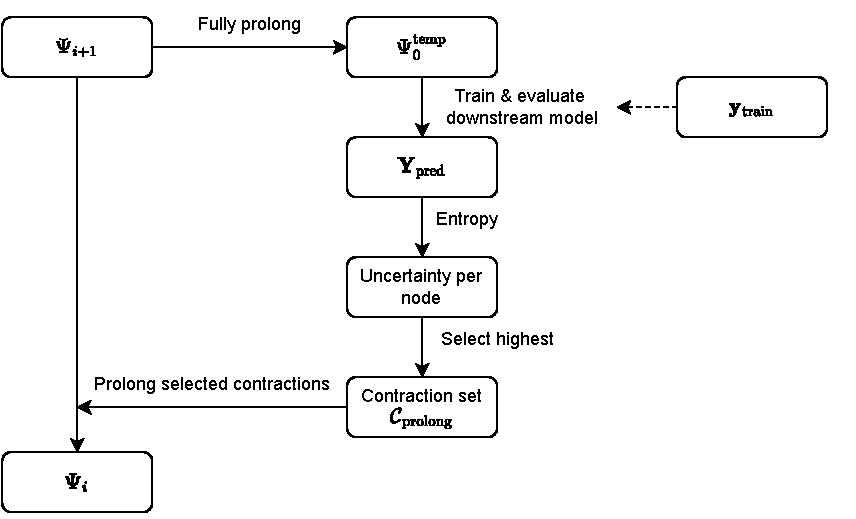
\includegraphics[width=0.45\textwidth]{images/adaptive-prolongation/adaptive-prolongation.pdf}
    \caption{A schematic explanation of the adaptive prolongation algorithm for obtaining the embedding \( \Phi_{G_{i - 1}} \) from \( \Phi_{G_i} \).}
  \label{fig:adaptive-prolongation}
\end{figure}

\begin{algorithm*}
  \caption{Adaptive prolongation}
  \label{alg:adaptive-prolongation}
  \begin{algorithmic}
    \Require $ G $ \Comment The original graph
    \Require $ \mathvec{e}_{i+1} $ \Comment The previous embedding
    \Require $ \mathvec{y}_\mathrm{train} $ \Comment Training labels
    \Require $ coarsening\_maps $ \Comment A list of all the original graph coarsenings
    \Require $ n_p $ \Comment The number of nodes to prolong
    \Ensure $ merges\_to\_prolong $ \Comment A list of node merges to be prolonged (\enquote{undone})
    \Ensure $ new\_coarsening\_maps $ \Comment Updated coarsening records without the prolonged merges
    \Statex
    \State $ node\_order \gets \Call{get\_node\_order}{G, \bm{e}_{i+1}, \bm{y}_\mathrm{train}, coarsening\_maps} $
    \State $ merges\_to\_prolong \gets \Call{select\_merges}{node\_order, n_p, coarsening\_maps} $
    \State $ new\_coarsening\_maps \gets \Call{undo\_merges}{coarsening\_maps, merges\_to\_prolong} $
    \Statex
    \Function{get\_node\_order}{$ G, \bm{e}_{i+1}, \bm{y}_\mathrm{train}, coarsening\_maps $}
        \State $ \bm{e}_0^\mathrm{temp} \gets $ use $ coarsening\_maps $ to fully prolong the current embedding $ \bm{e}_{i+1} $ to $ G_0 $
        \State $ model \gets \Call{train\_downstream\_model}{\bm{e}_0^\mathrm{temp}, \bm{y}_\mathrm{train}} $
        \State $ entropy\_per\_node \gets H \left( \Call{predict}{model, node} \right) $ for each $ node \in V \left( G \right) $
        \State \Return $ V \left( G \right) $, sorted in descending order by $ entropy\_per\_node $
    \EndFunction
    \Statex
    \Function{select\_merges}{$ ordered\_nodes, n_p, coarsening\_maps $}
        \State $ selected\_merges \gets \left\{ \right\} $
        \For{$ node \in ordered\_nodes $, \textbf{until} $ \left\lvert selected\_merges \right\rvert = n_p $}
            \State $ merge \gets \Call{resolve\_merge}{node, selected\_merges, coarsening\_maps} $
            \State If $ merge \neq \mathrm{null} $, add $ merge $ to $ selected\_merges $
        \EndFor
        \State \Return $ selected\_merges $
    \EndFunction
    \Statex
    \Function{resolve\_merge}{$ node, already\_selected\_merges, coarsening\_maps $}
        \State $ merge \gets \mathrm{null} $
        \For{$ coarsening\_map \in coarsening\_maps $ from finest graph to coarsest}
            \State $ merge\_candidate \gets $ find in $ coarsening\_map $ a merge that affects $ node $, if not found, continue with next $ coarsening\_map $
            \If{$ merge\_candidate \in already\_selected\_merges $}
                \State \Return $ merge $
            \EndIf
            \State $ merge \gets merge\_candidate $
            \State Apply $ merge $ to $ node $, so that in the next loop, a subsequent merge may be selected
        \EndFor
        \State \Return $ merge $
    \EndFunction
  \end{algorithmic}
\end{algorithm*}

The adaptive prolongation approach (Figure~\ref{fig:adaptive-prolongation}, Algorithm~\ref{alg:adaptive-prolongation}) uses the pre-computed coarsened graphs as a way to progressively increase the number of nodes with which the embedding is trained. However, its iterations of embedding training and prolongation are decoupled from the pre-computed coarsened graphs. Instead, in each step of the training, the current embedding is used to train a node classifier that guides which nodes should be prolonged. The node classifier is equivalent to the one which is to be eventually used for the downstream task and is trained on the same training subset of graph nodes. A measure guiding the prolongation is to be produced using this classifier -- ideally, only the nodes where the classifier performs the worst should be prolonged. To this end, the entropy of the probability distribution in the softmax layer for each node is used -- this represents the amount of uncertainty in the classifier for the given node. For each node, starting with nodes with the highest entropy, all of the pre-computed coarsenings are searched for edge contractions involving the node, with preference for contractions from later steps of the repeated coarsening (corresponding to coarser graphs). A given number of such edge contractions is selected and undone in each prolongation step, gradually advancing from the coarsest graph to the original, finest one.

\subsection{More general approaches to coarsening}\label{sec:coarsening-algorithms}

While the adaptive prolongation approach substantially generalizes the original method into a powerful tool for studying and leveraging graph structure and its properties under a coarsening, it still relies on the pre-computed coarsenings to guide the prolongation process. Moreover, the general coarsening schema described in Section~\ref{sec:coarsening-properties} and its variants described in this section are useful even beyond the methods proposed in this work. In this section, we first present a brief overview of the coarsening algorithm as proposed by \cite{chen_harp_2018}, followed by two alternative proposals for coarsening construction.

\subsubsection{HARP coarsening}\label{sec:harp-coarsening}

The authors of \cite{chen_harp_2018} introduce two particular coarsening methods that together realize the function \( \varphi_i \) from Section~\ref{sec:harp} -- \name{edge collapsing} and \name{star collapsing}. Edge collapsing is a very simple method -- out of all the edges \( E \left( G \right) \), a maximal subset \( E' \) is selected randomly such that no two edges from \( E' \) are incident on the same node. Then, each edge in \( E' \) is contracted.

The edge collapsing algorithm is a good general way of lowering the number of nodes in a graph. However, some structures are not easily collapsed by it. An example of such a structure is a \enquote{star} -- a single node connected to many other nodes. To coarsen graphs with such structures effectively, the star collapsing algorithm is proposed. For each such \textit{hub} node \( u \) in order of decreasing degree, its unconnected neighbouring nodes are taken and merged pairwise. All edges incident on such nodes are replaced with edges incident on the corresponding newly created nodes. As in edge collapsing, nodes to be merged are selected in such a way that no node is merged twice.

These two approaches are combined in the original HARP method, with each coarsening step being a star collapsing step followed by an edge collapsing step. Of a particular note is the fact such a coarsening scheme is not in agreement with the definition presented in Section~\ref{sec:coarsening-properties}. The star collapsing algorithm merges nodes that are adjacent to a common hub node, however, these nodes need not be connected by an edge. In our previous work \cite{dedic_graph_2021}, we experimentally verified that the star collapsing algorithm can be replaced by a similar algorithm that repeatedly merges nodes adjacent on a hub node with the hub node itself. Such a replacement modifies the HARP coarsening scheme to be in line with the definition presented in Section~\ref{sec:coarsening-properties}.

\subsubsection{Graph diffusion coarsening}\label{sec:gdc-coarsening}

Our definition of a graph coarsening requires choosing some edges from the original graph. Intuitively, one way of constructing a graph coarsening would be to merge nodes which are similar and therefore no significant amount of information is lost due to such a coarsening. Following both of these premises, we propose a coarsening based on Graph Diffusion Convolution (GDC) \cite{gasteiger_diffusion_2019} algorithm. GDC is a general graph transformation which, in an overview, constructs for a given graph a new edge set, represented by a so-called sparsified generalized graph diffusion matrix \( \hat{\mathmat{S}} \), which would, in the original setting of the method, be used as a replacement for the adjacency matrix of the graph. To apply this algorithm as a way of coarsening the graph, the edge set obtained by GDC is intersected with the edges of the original graph and the resulting edges contracted in the graph, i.e.,
\[ \mathcal{C} = E \left( G_{\hat{\mathmat{S}}} \right) \cap E \left( G \right), \]
using the notation of a general graph coarsening presented in Section~\ref{sec:coarsening-properties}.

In principle, the authors of GDC define the generalized graph diffusion matrix
\begin{equation}\label{eq:gdc-matrix}
    \mathmat{S} = \sum_{k = 1}^\infty \theta_k \mathmat{T}^k
\end{equation}
such that the power series converges. The parameters \( \theta_k \) together with the generalized transition matrix \( \mathmat{T} \) define the exact way in which the diffusion is achieved. Among the choices for \( \mathmat{T} \) is the random walk transition matrix \( \mathmat{T}_ \mathrm{rw} = \mathmat{A} \mathmat{D}^{-1} \) and the symmetric transition matrix \( \mathmat{T}_\mathrm{sym} = \mathmat{D}^{-\frac{1}{2}} \mathmat{A} \mathmat{D}^{-\frac{1}{2}} \) where \( \mathmat{D} \) is the diagonal matrix of node degrees. Two special cases of this general schema using the random walk transition matrix are the Personalized PageRank algorithm (PPR) \cite{page_pagerank_1999} and the heat kernel \cite{kondor_diffusion_2002}. PPR corresponds to choosing
\[ \theta_k = \alpha \left( 1 - \alpha \right)^k \]
where the parameter \( \alpha \in \left( 0, 1 \right) \) is called the teleport probability. The heat kernel corresponds to choosing
\[ \theta_k = e^{-t} \frac{t^k}{k!} \]
with the parameter \( t \) being called the diffusion time. For both of these special cases, Equation \ref{eq:gdc-matrix} has a closed-form solution.

The result of most diffusion processes (including PPR and the heat kernel) is a dense matrix \( \mathmat{S} \), which then needs to be sparsified. In GDC, two methods of sparsification are considered -- thresholding the matrix values and selecting top-\( k \) entries for each column of the matrix. In any case, the matrix is normalized after sparsification, thus finally producing \( \hat{\mathmat{S}} \).

\subsubsection{Evolved coarsening}

The idea behind the evolutionary coarsening algorithm is to find a coarsening providing a good trade-off between the performance and complexity of the downstream task by searching through a space of graph coarsenings composed of elementary (atomic) coarsenings, each of which contracts \( O(1) \) edges. This search is performed using a simple evolutionary algorithm.

Let \( \mathspace{AC} \) be a basis of \name{atomic coarsenings}, \( \mathspace{AC} = \left\{\psi_i, i \in \left\{1, \dots, K \right\} \right\} \) for some \( K \in \mathfield{N} \), where each \( \psi_i \) is a function of a hyper-parameter vector \( \theta_i \) and of a graph \( G \) (See Table~\ref{tab:atomic-coarsenings} for examples of such atomic coarsenings). For the sake of simplicity, we will assume that in the course of an optimization run, each \( \psi_i \) is already partially applied to a particular fixed value of its hyper-parameters \( \theta_i \) and thus is a function of a graph only.

Each candidate solution \( \mathvec{x} = \left( j_i \right)_{i = 1}^L, j_i \in \left\{1, \dots, K \right\} \) is a sequence of \( L \) integers (genes), where the length \( L \) depends only on the graph size. The genome encodes a transformation \( \varphi_{\mathvec{x}} = \psi_{j_0} \cdot \psi_{j_1} \cdot \ldots \cdot \psi_{j_L} \) of the input graph \( G \), where \( \cdot \) denotes function composition.

The fitness \( f \left( \mathvec{x} \right) \), i.e. the objective function, is the classification accuracy of the downstream task on the validation subset of the graph \( \varphi_{\mathvec{x}} \left( G \right) \).

The evolutionary coarsening algorithm is a simple genetic algorithm. The offspring population is generated by the mutation and crossover operators. The crossover operator is a two-point crossover. The mutation of a single gene is a uniform choice from the index set of \( \mathspace{AC} \). Both the mutation and the crossover operators preserve the candidate solution length. The selection is a standard tournament selection. To compute the fitness, the graph is passed through the composite coarsening defined by each candidate solution.
